\documentclass[11pt]{article}

\usepackage[letterpaper,margin=1in]{geometry}

% ToC
\usepackage{blindtext} 
\usepackage[linktocpage]{hyperref}
\usepackage{bookmark}
\usepackage{titlesec}

% bib
%\usepackage[round]{natbib}
\usepackage[square,sort,numbers]{natbib}

% Math Imports
\usepackage{amsmath, amssymb, bm, fancyhdr, sectsty, dsfont, mathtools}

% Tikz
\usepackage{tikz}
\usetikzlibrary{bayesnet}
\usetikzlibrary{arrows}

\usepackage{wrapfig}
\usepackage{comment}
\usepackage{subcaption}

% Symbols
\newcommand\ind{\protect\mathpalette{\protect\independenT}{\perp}}
\def\independenT#1#2{\mathrel{\rlap{$#1#2$}\mkern2mu{#1#2}}}
\newcommand\norm[1]{\left\lVert#1\right\rVert}
\newcommand\set[1]{\left\{#1\right\}}

\newcommand\RNN{\mathrm{RNN}}
\newcommand\MLP{\mathrm{MLP}}
\newcommand\enc{\mathrm{enc}}
\newcommand\softmax{\mathrm{softmax}}

% Distributions
\newcommand{\Cat}{\mathrm{Cat}}
\newcommand\Expo{\mathrm{Expo}}
\newcommand\Bern{\mathrm{Bern}}
\newcommand\Pois{\mathrm{Pois}}
\newcommand\Bin{\mathrm{Bin}}
\newcommand\Unif{\mathrm{Unif}}
\newcommand\Betad{\mathrm{Beta}}
\newcommand\Gammad{\mathrm{Gamma}}
\newcommand\Geom{\mathrm{Geom}}
\newcommand\Logd{\mathrm{Logistic}}

\newcommand\E[1]{\mathbb{E}\left[#1\right]}
\newcommand\Es[2]{\mathbb{E}_{#1}\left[#2\right]}
\newcommand{\Var}{\mathrm{Var}}
\newcommand{\Cov}{\mathrm{Cov}}
\newcommand{\Cor}{\mathrm{Cor}}

% Bold stuff
\newcommand{\ba}{\mathbf{a}}
\newcommand{\bb}{\mathbf{b}}
\newcommand{\bc}{\mathbf{c}}
\newcommand{\bd}{\mathbf{d}}
\newcommand{\be}{\mathbf{e}}
\newcommand{\bg}{\mathbf{g}}
\newcommand{\bh}{\mathbf{h}}
\newcommand{\br}{\mathbf{r}}
\newcommand{\bs}{\mathbf{s}}
\newcommand{\bw}{\mathbf{w}}
\newcommand{\bx}{\mathbf{x}}
\newcommand{\by}{\mathbf{y}}
\newcommand{\bz}{\mathbf{z}}

% mathcal stuff
\newcommand{\mcD}{\mathcal{D}}

% math blackboard bold stuff
\newcommand{\R}{\mathbb{R}}
\newcommand{\C}{\mathbb{C}}
\newcommand{\Z}{\mathbb{Z}}
\newcommand{\N}{\mathbb{N}}
\newcommand{\Q}{\mathbb{Q}}


\DeclareMathOperator*{\argmin}{argmin}
\DeclareMathOperator*{\argmax}{argmax}

\usepackage{fancyhdr}
\pagestyle{fancy}

\begin{document}
\lhead{Justin Chiu}
\chead{2018 NSF GRFP}
\rhead{Research Proposal}

\section{Background}
Natural language processing (NLP) can largely be decomposed into two separate but
tightly related tasks: natural language understanding and natural language generation (NLG).
In this proposal we focus primarily on text generation, and in particular
the generation of text that describes some data.
We refer to this specific task as Data-to-Text (D2T).

\section{What exactly is D2T?}
An example of D2T is in \citet{wiseman2017d2t},
where a summary of a basketball game is modelled conditioned on
the box score associated with that game.
The box score consists of a list of records associating an entity with a value.
Each record has a type which denotes the relationship between the entity and value contained in the record.

\section{Why is D2T important?}
% Easily evaluable, good benchmark
% Limited external knowledge
% Largely concerned with reporting the information in the table
The D2T task's importance is two-fold.
First, D2T serves as a benchmark for conditional generation.
D2T exists as a compromise between short-form generative tasks such as sentence-level translation
and unstructured long-form tasks such as generating Wikipedia articles from sources and search results.
This is because D2T is a long-form generation task but uses structured data as input instead of free-form text.
The existence of structured data represents a simplifying assumption which makes D2T easier than other
long-form tasks but also more evaluable.

% Proposal? Add more structure / modularity, principled inference...?
Early work on text generation focused on the use of templates and grammars, 
which generally resulted in generations with little stylistic variation.
% Do I need to qualify this claim and say why?
After neural language models demonstrated state of the art performance,
they were then transferred to the conditional language modeling setting,
i.e. NLG,
where they supplanted template-based methods almost completely.
However, by relying largely on the language modeling capabilities of neural networks,
practitioners have eschewed modularity of the model for ease of inference.
% Do I need to qualify this as well?

\section{What are the desiderata of a text generation system?}
\begin{enumerate}
\item Readability: Fluency, grammaticality, interestingness?
\item Controllability, ability to impose constraints
\item Fidelity to conditioning
\item What does interpretability mean here?
\item Informational adequacy: Can we learn what records are salient?
\end{enumerate}

A vein in the recent work on integrating neural network systems and latent variable models
has aimed to separate content from style.

Separate style and content, where content will come from for controllable generation.
Can we also model intention in a similar way?
Hierarchical planning, multiple levels
cite 
\section{Related Work}
In the task of generating basketball summaries from game statistics,
\citet{puduppully2018contentselection} learn a model of content progression
by learning how to order records from the table of statistics.
\citep{puduppully2018contentselection,wiseman2018template}
Separate content from style
\section{Research Question}
Given that we can model `what to say' as well as `how to say',
can we learn a model of intention?
\section{Keywords}
\section{Approach and Methods}
\begin{figure}[ht]
\centering
\begin{subfigure}[]{0.3\textwidth}
\centering
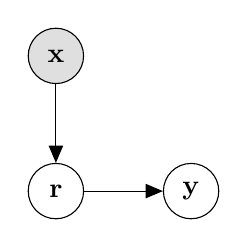
\begin{tikzpicture}
\node(x)[obs]{$\bx$};
\node(r)[latent, below =of x]{$\br$};
\node(y)[latent, right =of r]{$\by$};
\edge {x} {r};
\edge {r} {y};
\end{tikzpicture}
\caption{}
\end{subfigure}

\hspace{0.03\textwidth}
\begin{subfigure}[]{0.3\textwidth}
\centering
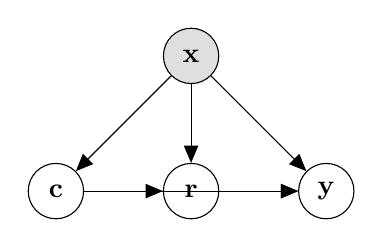
\begin{tikzpicture}
\node(x)[obs]{$\bx$};
\node(r)[latent, below =of x]{$\br$};
\node(c)[latent, left =of r]{$\bc$};
\node(y)[latent, right =of r]{$\by$};

\edge {x} {c};
\edge {x} {r};
\edge {x} {y};
\edge {c} {r};
\edge [bend right=45] {c} {y};
\edge {r} {y};

\end{tikzpicture}
\caption{}
\end{subfigure}
\hspace{0.03\textwidth}

\begin{comment}
% Noisy channel model
\begin{subfigure}[]{0.3\textwidth}
\centering
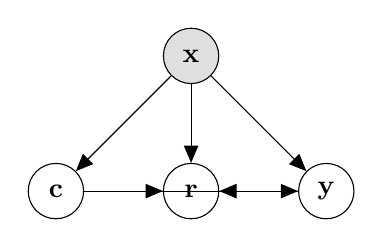
\begin{tikzpicture}
\node(x)[obs]{$\bx$};
\node(r)[latent, below =of x]{$\br$};
\node(c)[latent, left =of r]{$\bc$};
\node(y)[latent, right =of r]{$\by$};

\edge {x} {c};
\edge {x} {r};
\edge {x} {y};
\edge {c} {r};
\edge [bend right=45] {c} {y};
\edge {y} {r};
\end{tikzpicture}
\caption{}
\end{subfigure}
\end{comment}

\begin{subfigure}[]{0.3\textwidth}
\centering
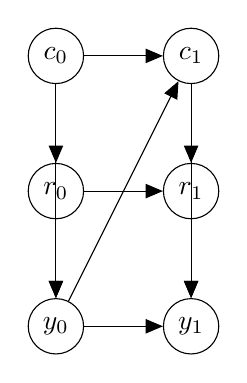
\begin{tikzpicture}
\node(c0)[latent]{$c_0$};
\node(r0)[latent, below =of c0]{$r_0$};
\node(y0)[latent, below =of r0]{$y_0$};
\node(c1)[latent, right =of c0]{$c_1$};
\node(r1)[latent, below =of c1]{$r_1$};
\node(y1)[latent, below =of r1]{$y_1$};

\edge {c0} {r0};
\edge [bend right=45] {c0} {y0};
\edge {r0} {y0};

\edge {c1} {r1};
\edge [bend left=45] {c1} {y1};
\edge {r1} {y1};

\edge {c0} {c1};
\edge {r0} {r1};
\edge {y0} {y1};

\edge {y0} {c1};

\end{tikzpicture}
\caption{}
\end{subfigure}
\label{fig:dgm}
\caption{Simplistic directed graphical models for the latent variable model.
The observed context is $\tilde\bx$, current attention $a_t$, previous attention $a_{t-1}$,
state $s_t$, and target word $y_t$.}
\end{figure}

\begin{figure}[ht]
\label{fig:dgm2}
\caption{The time-series graphical model.
As all nodes condition on $\bx$, we omit it from the diagram.}
\end{figure}

\section{Intellectual Merit}
\section{Broader Impact}


\bibliographystyle{plainnat}
\bibliography{w}


\end{document}

